\hypertarget{times-and-places}{%
\chapter{Times and places}\label{times-and-places}}

In the previous chapter, you learned about variables and two kinds of
values: integers and floating-point numbers.

In this chapter, you'll see some additional types:

\begin{itemize}
\item
  Strings, which represent text.
\item
  Time stamps, which represent dates and times.
\item
  And several ways to represent and display geographical locations.
\end{itemize}

Not every data science project uses all of these types, but many
projects use at least one.

\hypertarget{strings}{%
\section{Strings}\label{strings}}

A \textbf{string} is a sequence of letters, numbers, and punctuation
marks. In Python you can create a string by typing letters between
single or double quotation marks.

\begin{lstlisting}[language=Python,style=source]
'Elements'
\end{lstlisting}

\begin{lstlisting}[style=output]
'Elements'
\end{lstlisting}

\begin{lstlisting}[language=Python,style=source]
"of"
\end{lstlisting}

\begin{lstlisting}[style=output]
'of'
\end{lstlisting}

And you can assign string values to variables.

\begin{lstlisting}[language=Python,style=source]
first = 'Data'
\end{lstlisting}

\begin{lstlisting}[language=Python,style=source]
last = "Science"
\end{lstlisting}

Some arithmetic operators work with strings, but they might no do what
you expect. For example, the \passthrough{\lstinline!+!} operator
``concatenates'' two strings; that is, it creates a new string that
contains the first string followed by the second string:

\begin{lstlisting}[language=Python,style=source]
first + last
\end{lstlisting}

\begin{lstlisting}[style=output]
'DataScience'
\end{lstlisting}

If you want to put a space between the words, you can use a string that
contains a space:

\begin{lstlisting}[language=Python,style=source]
first + ' ' + last
\end{lstlisting}

\begin{lstlisting}[style=output]
'Data Science'
\end{lstlisting}

Strings are used to store text data like names, addresses, titles, etc.

When you read data from a file, you might see values that look like
numbers, but they are actually strings, like this:

\begin{lstlisting}[language=Python,style=source]
not_actually_a_number = '123'
\end{lstlisting}

If you try to do math with these strings, you \emph{might} get an error.
For example, the following expression causes a
\passthrough{\lstinline!TypeError!} with the message ``can only
concatenate \passthrough{\lstinline!str!} (not
\passthrough{\lstinline!int!}) to \passthrough{\lstinline!str!}''.

\begin{lstlisting}[style=output]
not_actually_a_number + 1
\end{lstlisting}

But you don't always get an error; instead, you might get a surprising
result. For example:

\begin{lstlisting}[language=Python,style=source]
not_actually_a_number * 3
\end{lstlisting}

\begin{lstlisting}[style=output]
'123123123'
\end{lstlisting}

If you multiply a string by an integer, Python repeats the string the
given number of times.

If you have a string that contains only digits, you can convert it to an
integer using the \passthrough{\lstinline!int!} function:

\begin{lstlisting}[language=Python,style=source]
int('123')
\end{lstlisting}

\begin{lstlisting}[style=output]
123
\end{lstlisting}

Or you can convert it to a floating-point number using
\passthrough{\lstinline!float!}:

\begin{lstlisting}[language=Python,style=source]
float('123')
\end{lstlisting}

\begin{lstlisting}[style=output]
123.0
\end{lstlisting}

But if the string contains a decimal point, you can't convert it to an
\passthrough{\lstinline!int!}.

Going in the other direction, you can convert any type of value to a
string using \passthrough{\lstinline!str!}:

\begin{lstlisting}[language=Python,style=source]
str(123)
\end{lstlisting}

\begin{lstlisting}[style=output]
'123'
\end{lstlisting}

\begin{lstlisting}[language=Python,style=source]
str(12.3)
\end{lstlisting}

\begin{lstlisting}[style=output]
'12.3'
\end{lstlisting}

\textbf{Exercise}: When personal names are stored in a database, they
are often stored in three variables: a given name, a family name, and
sometimes a middle name. For example, a list of great rock drummers
might include:

\begin{lstlisting}[language=Python,style=source]
given = 'Neil'
middle = 'Ellwood'
family = 'Peart'
\end{lstlisting}

But names are often displayed different ways in different contexts. For
example, the first time you mention someone in an article, you might
give all three names, like ``Neil Ellwood Peart''. But in the index of a
book, you might put the family name first, like ``Peart, Neil Ellwood''.

Write Python expressions that use the variables
\passthrough{\lstinline!given!}, \passthrough{\lstinline!middle!}, and
\passthrough{\lstinline!family!} to display Neil Peart's name in these
two formats.

\hypertarget{dates-and-times}{%
\section{Dates and times}\label{dates-and-times}}

If you read data from a file, you might also find that dates and times
are represented with strings.

\begin{lstlisting}[language=Python,style=source]
not_really_a_date = 'June 4, 1989'
\end{lstlisting}

To confirm that this value is a string, we can use the
\passthrough{\lstinline!type!} function, which takes a value and reports
its type.

\begin{lstlisting}[language=Python,style=source]
type(not_really_a_date)
\end{lstlisting}

\begin{lstlisting}[style=output]
str
\end{lstlisting}

\passthrough{\lstinline!str!} indicates that the value of
\passthrough{\lstinline!not\_really\_a\_date!} is a string.

We get the same result with
\passthrough{\lstinline!not\_really\_a\_time!}, below:

\begin{lstlisting}[language=Python,style=source]
not_really_a_time = '6:30:00'
type(not_really_a_time)
\end{lstlisting}

\begin{lstlisting}[style=output]
str
\end{lstlisting}

Strings that represent dates and times a readable for people, but they
are not useful for computation.

Fortunately, Python provides libraries for working with date and time
data; the one we'll use is called Pandas. As always, we have to import a
library before we use it; it is conventional to import Pandas with the
abbreviated name \passthrough{\lstinline!pd!}:

\begin{lstlisting}[language=Python,style=source]
import pandas as pd
\end{lstlisting}

Pandas provides a type called \passthrough{\lstinline!Timestamp!}, which
represents a date and time.

It also provides a function called \passthrough{\lstinline!Timestamp!},
which we can use to convert a string to a
\passthrough{\lstinline!Timestamp!}:

\begin{lstlisting}[language=Python,style=source]
pd.Timestamp('6:30:00')
\end{lstlisting}

\begin{lstlisting}[style=output]
Timestamp('2021-05-11 06:30:00')
\end{lstlisting}

Or we can do the same thing using the variable defined above.

\begin{lstlisting}[language=Python,style=source]
pd.Timestamp(not_really_a_time)
\end{lstlisting}

\begin{lstlisting}[style=output]
Timestamp('2021-05-11 06:30:00')
\end{lstlisting}

In this example, the string specifies a time but no date, so Pandas
fills in today's date.

A \passthrough{\lstinline!Timestamp!} is a value, so you can assign it
to a variable.

\begin{lstlisting}[language=Python,style=source]
date_of_birth = pd.Timestamp('June 4, 1989')
date_of_birth
\end{lstlisting}

\begin{lstlisting}[style=output]
Timestamp('1989-06-04 00:00:00')
\end{lstlisting}

If the string specifies a date but no time, Pandas fills in midnight as
the default time.

If you assign the \passthrough{\lstinline!Timestamp!} to a variable, you
can use the variable name to get the year, month, and day, like this:

\begin{lstlisting}[language=Python,style=source]
date_of_birth.year, date_of_birth.month, date_of_birth.day
\end{lstlisting}

\begin{lstlisting}[style=output]
(1989, 6, 4)
\end{lstlisting}

You can also gets the name of the month and the day of the week.

\begin{lstlisting}[language=Python,style=source]
date_of_birth.day_name(), date_of_birth.month_name()
\end{lstlisting}

\begin{lstlisting}[style=output]
('Sunday', 'June')
\end{lstlisting}

\passthrough{\lstinline!Timestamp!} provides a function called
\passthrough{\lstinline!now!} that returns the current date and time.

\begin{lstlisting}[language=Python,style=source]
now = pd.Timestamp.now()
now
\end{lstlisting}

\begin{lstlisting}[style=output]
Timestamp('2021-05-11 10:46:54.137321')
\end{lstlisting}

\textbf{Exercise:} Use the value of \passthrough{\lstinline!now!} to
display the name of the current month and day of the week.

\hypertarget{timedelta}{%
\section{Timedelta}\label{timedelta}}

\passthrough{\lstinline!Timestamp!} values support some arithmetic
operations. For example, you can compute the difference between two
\passthrough{\lstinline!Timestamps!}:

\begin{lstlisting}[language=Python,style=source]
age = now - date_of_birth
age
\end{lstlisting}

\begin{lstlisting}[style=output]
Timedelta('11664 days 10:46:54.137321')
\end{lstlisting}

The result is a \passthrough{\lstinline!Timedelta!} that represents the
current age of someone born on
\passthrough{\lstinline!date\_of\_birth!}. The
\passthrough{\lstinline!Timedelta!} contains
\passthrough{\lstinline!components!} that store the number of days,
hours, etc. between the two \passthrough{\lstinline!Timestamp!} values.

\begin{lstlisting}[language=Python,style=source]
age.components
\end{lstlisting}

\begin{lstlisting}[style=output]
Components(days=11664, hours=10, minutes=46, seconds=54, milliseconds=137, microseconds=321, nanoseconds=0)
\end{lstlisting}

You can get one of the components like this:

\begin{lstlisting}[language=Python,style=source]
age.days
\end{lstlisting}

\begin{lstlisting}[style=output]
11664
\end{lstlisting}

The biggest component of \passthrough{\lstinline!Timedelta!} is days,
not years, because days are well defined and years are problematic.

Most years are 365 days, but some are 366. The average calendar year is
365.24 days, which is a very good approximation of a solar year,
\href{https://pumas.jpl.nasa.gov/files/04_21_97_1.pdf}{but it is not
exact}.

One way to compute age in years is to divide age in days by 365.24:

\begin{lstlisting}[language=Python,style=source]
age.days / 365.24
\end{lstlisting}

\begin{lstlisting}[style=output]
31.935165918300296
\end{lstlisting}

But people usually report their ages in integer years. We can use the
Numpy \passthrough{\lstinline!floor!} function to round down:

\begin{lstlisting}[language=Python,style=source]
import numpy as np

np.floor(age.days / 365.24)
\end{lstlisting}

\begin{lstlisting}[style=output]
31.0
\end{lstlisting}

Or the \passthrough{\lstinline!ceil!} function (which stands for
``ceiling'') to round up:

\begin{lstlisting}[language=Python,style=source]
np.ceil(age.days / 365.24)
\end{lstlisting}

\begin{lstlisting}[style=output]
32.0
\end{lstlisting}

We can also compare \passthrough{\lstinline!Timestamp!} values to see
which comes first. For example, let's see if a person with a given
birthdate has already had a birthday this year. Here's a new
\passthrough{\lstinline!Timestamp!} with the year from
\passthrough{\lstinline!now!} and the month and day from
\passthrough{\lstinline!date\_of\_birth!}.

\begin{lstlisting}[language=Python,style=source]
bday_this_year = pd.Timestamp(now.year, 
                              date_of_birth.month, 
                              date_of_birth.day)
bday_this_year
\end{lstlisting}

\begin{lstlisting}[style=output]
Timestamp('2021-06-04 00:00:00')
\end{lstlisting}

The result represents the person's birthday this year. Now we can use
the \passthrough{\lstinline!>!} operator to check whether
\passthrough{\lstinline!now!} is later than the birthday:

\begin{lstlisting}[language=Python,style=source]
now > bday_this_year
\end{lstlisting}

\begin{lstlisting}[style=output]
False
\end{lstlisting}

The result is either \passthrough{\lstinline!True!} or
\passthrough{\lstinline!False!}. These values belong to a type called
\passthrough{\lstinline!bool!}, short for ``Boolean algebra'', which is
a branch of algebra where all values are either true or false.

\begin{lstlisting}[language=Python,style=source]
type(True)
\end{lstlisting}

\begin{lstlisting}[style=output]
bool
\end{lstlisting}

\begin{lstlisting}[language=Python,style=source]
type(False)
\end{lstlisting}

\begin{lstlisting}[style=output]
bool
\end{lstlisting}

\textbf{Exercise:} Any two people with different birthdays have a
``Double Day'' when one is twice as old as the other. Suppose you are
given two \passthrough{\lstinline!Timestamp!} values,
\passthrough{\lstinline!d1!} and \passthrough{\lstinline!d2!}, that
represent birthdays for two people. Use
\passthrough{\lstinline!Timestamp!} arithmetic to compute their double
day. With the following dates, the result should be December 19, 2009.

\begin{lstlisting}[language=Python,style=source]
d1 = pd.Timestamp('2003-07-12')
d2 = pd.Timestamp('2006-09-30')
\end{lstlisting}

\hypertarget{location}{%
\section{Location}\label{location}}

There are many ways to represent geographical locations, but the most
common, at least for global data, is latitude and longitude.

When stored as strings, latitude and longitude are expressed in degrees
with compass directions N, S, E, and W. For example, this string
represents the location of Boston, MA, USA:

\begin{lstlisting}[language=Python,style=source]
lat_lon_string = '42.3601° N, 71.0589° W'
\end{lstlisting}

When we compute with location information, we use floating-point
numbers, with

\begin{itemize}
\item
  Positive latitude for the northern hemisphere, negative latitude for
  the southern hemisphere, and
\item
  Positive longitude for the eastern hemisphere and negative latitude
  for the western hemisphere.
\end{itemize}

Of course, the choice of the origin and the orientation of positive and
negative are arbitrary choices that were made for historical reasons. We
might not be able to change conventions like these, but we should be
aware that they are conventions.

Here's how we might represent the location of Boston with two variables.

\begin{lstlisting}[language=Python,style=source]
lat = 42.3601
lon = -71.0589
\end{lstlisting}

It is also possible to combine two numbers into a composite value and
assign it to a single variable:

\begin{lstlisting}[language=Python,style=source]
boston = lat, lon
boston
\end{lstlisting}

\begin{lstlisting}[style=output]
(42.3601, -71.0589)
\end{lstlisting}

The type of this variable is \passthrough{\lstinline!tuple!}, which is a
mathematical term for a value that contains a sequence of elements. Math
people pronounce it ``tuh' ple'', but computational people usually say
``too' ple''. Take your pick.

\begin{lstlisting}[language=Python,style=source]
type(boston)
\end{lstlisting}

\begin{lstlisting}[style=output]
tuple
\end{lstlisting}

If you have a tuple with two elements, you can assign them to two
variables, like this:

\begin{lstlisting}[language=Python,style=source]
y, x = boston
y
\end{lstlisting}

\begin{lstlisting}[style=output]
42.3601
\end{lstlisting}

\begin{lstlisting}[language=Python,style=source]
x
\end{lstlisting}

\begin{lstlisting}[style=output]
-71.0589
\end{lstlisting}

Notice that I assigned latitude to \passthrough{\lstinline!y!} and
longitude to \passthrough{\lstinline!x!}, because a
\passthrough{\lstinline!y!} coordinate usually goes up and down like
latitude, and an \passthrough{\lstinline!x!} coordinate usually goes
side-to-side like longitude.

\textbf{Exercise:} Find the latitude and longitude of the place you were
born or someplace you think of as your ``home town''.
\href{https://www.latlong.net/}{You can use this web page to look it
up}. Make a tuple of floating-point numbers that represents that
location.

\hypertarget{distance}{%
\section{Distance}\label{distance}}

If you are given two tuples that represent locations, you can compute
the approximate distance between them, along the surface of the globe,
using the haversine function. If you are curious about it,
\href{https://janakiev.com/blog/gps-points-distance-python/}{you can
read an explanation in this article}. To estimate a haversine distance,
we have to compute the haversine function, which is defined:

\(\mathrm{haversine}(\theta)=\sin^2(\theta/2)\)

Where \(\theta\) is an angle in radians. We can compute this function in
Python like this:

\begin{lstlisting}[language=Python,style=source]
import numpy as np

θ = 1
np.sin(θ/2)**2
\end{lstlisting}

\begin{lstlisting}[style=output]
0.22984884706593015
\end{lstlisting}

You can use Greek letters in variable names, but there is currently no
way to type them in Jupyter/Colab, so I usually copy them from a web
page and paste them in.

To avoid the inconvenience, it is more common to write out letter names,
like this:

\begin{lstlisting}[language=Python,style=source]
theta = 1
np.sin(theta/2)**2
\end{lstlisting}

\begin{lstlisting}[style=output]
0.22984884706593015
\end{lstlisting}

Remember that the operator for exponentiation is
\passthrough{\lstinline!**!}.\\
In some other languages it's \passthrough{\lstinline!\^!}, which is also
an operator in Python, but it performs another operation altogether.

\hypertarget{defining-functions}{%
\section{Defining functions}\label{defining-functions}}

At this point you don't have to know how to define a new function. But
you will see function definitions, so I want to explain the basics now.

If we are planning to use an expression like
\passthrough{\lstinline!np.sin(theta/2)**2!} more than a few times, we
can define a new function that computes it, like this:

\begin{lstlisting}[language=Python,style=source]
def haversine(theta):
    """Compute the haversine function of theta."""
    return np.sin(theta/2)**2
\end{lstlisting}

On the first line, \passthrough{\lstinline!def!} indicates that we are
defining a function.

The second line is a ``triple-quoted string'', which describes what the
function does, but it has no effect when the program runs.

On the third line, \passthrough{\lstinline!return!} indicates the result
of the function.

When you run the previous cell, it creates a new variable called
\passthrough{\lstinline!haversine!}. You can display its value like
this:

\begin{lstlisting}[language=Python,style=source]
haversine
\end{lstlisting}

\begin{lstlisting}[style=output]
<function __main__.haversine(theta)>
\end{lstlisting}

And you can display its type like this:

\begin{lstlisting}[language=Python,style=source]
type(haversine)
\end{lstlisting}

\begin{lstlisting}[style=output]
function
\end{lstlisting}

So \passthrough{\lstinline!haversine!} is a variable that refers to a
function. To run the function and compute a result, we have to ``call''
the function and provide a value for \passthrough{\lstinline!theta!}:

\begin{lstlisting}[language=Python,style=source]
haversine(1)
\end{lstlisting}

\begin{lstlisting}[style=output]
0.22984884706593015
\end{lstlisting}

When you define a function, you create a new variable. But the function
doesn't actually run until you call it.

\hypertarget{haversine-distance}{%
\section{Haversine distance}\label{haversine-distance}}

Now we can use \passthrough{\lstinline!haversine!} as part of a function
that computes haversine distances. I won't explain this function in as
much detail, but if you read through it, you might get a sense of how it
works.

\begin{lstlisting}[language=Python,style=source]
def haversine_distance(coord1, coord2):
    """Haversine distance between two locations.
    
    coord1: lat-lon as tuple of float 
    coord2: lat-lon as tuple of float
    
    returns: distance in km
    """
    R = 6372.8  # Earth radius in km
    lat1, lon1 = coord1
    lat2, lon2 = coord2
    
    phi1, phi2 = np.radians(lat1), np.radians(lat2) 
    dphi       = np.radians(lat2 - lat1)
    dlambda    = np.radians(lon2 - lon1)
    
    a = haversine(dphi) + np.cos(phi1)*np.cos(phi2)*haversine(dlambda)
    
    distance = 2*R*np.arctan2(np.sqrt(a), np.sqrt(1 - a))
    
    return distance
\end{lstlisting}

When we call this function, we provide two tuples, each representing a
latitude and a longitude. We already have a tuple that represents the
location of Boston. Now here's a tuple that represents the location of
London, England, UK:

\begin{lstlisting}[language=Python,style=source]
london = 51.5074, -0.1278
\end{lstlisting}

And here's the haversine distance between Boston and London.

\begin{lstlisting}[language=Python,style=source]
haversine_distance(boston, london)
\end{lstlisting}

\begin{lstlisting}[style=output]
5265.656325981015
\end{lstlisting}

The actual geographic distance is slightly different because Earth is
not a perfect sphere. But the error of this estimate is less than 1\%.

\textbf{Exercise:} Use \passthrough{\lstinline!haversine\_distance!} to
compute the distance between Boston and your home town from the previous
exercise.

If possible, use an online map to check the result.

\hypertarget{geopandas}{%
\section{Geopandas}\label{geopandas}}

Python provides libraries for working with geographical data. One of the
most popular is Geopandas, which is based on another library called
Shapely. Shapely provides \passthrough{\lstinline!Point!} and
\passthrough{\lstinline!LineString!} values, which we'll use to
represent geographic locations and lines between them.

\begin{lstlisting}[language=Python,style=source]
from shapely.geometry import Point, LineString
\end{lstlisting}

We can use the tuples we defined in the previous section to create
Shapely \passthrough{\lstinline!Point!} values, but we have to reverse
the order of the coordinates, providing them in \(x\)-\(y\) order rather
than \passthrough{\lstinline!lat!}-\passthrough{\lstinline!lon!} order,
because that's the order the \passthrough{\lstinline!Point!} function
expects.

\begin{lstlisting}[language=Python,style=source]
lat, lon = boston
p1 = Point(lon, lat)
\end{lstlisting}

\begin{lstlisting}[language=Python,style=source]
lat, lon = london
p2 = Point(lon, lat)
\end{lstlisting}

We can use the points we just defined to create a
\passthrough{\lstinline!LineString!}:

\begin{lstlisting}[language=Python,style=source]
line = LineString([p1, p2])
\end{lstlisting}

Now we can use Geopandas to show these points and lines on a map. The
following code loads a map of the world and plots it.

\begin{lstlisting}[language=Python,style=source]
import geopandas as gpd

path = gpd.datasets.get_path('naturalearth_lowres')
world = gpd.read_file(path)
world.plot(color='white', edgecolor='gray');
\end{lstlisting}

\begin{center}
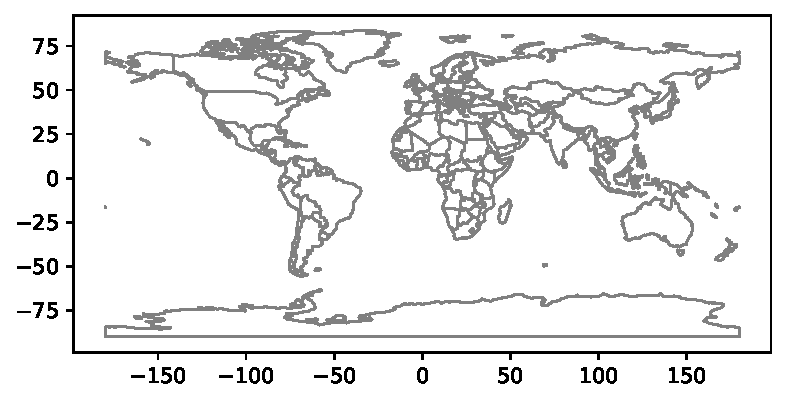
\includegraphics[scale=0.75]{02_times_files/02_times_123_0.pdf}
\end{center}

By default, Geopandas uses an equirectangular projection, which provides
a misleading picture of relative land areas (see
\url{https://en.wikipedia.org/wiki/Equirectangular_projection}). You
can't make a map without making visualization decisions.

Now let's put dots on the map for Boston and London. We have to put the
\passthrough{\lstinline!Point!} values and the
\passthrough{\lstinline!LineString!} into a
\passthrough{\lstinline!GeoSeries!}.

\begin{lstlisting}[language=Python,style=source]
t = [p1, p2, line]
series = gpd.GeoSeries(t)
\end{lstlisting}

Here's a first attempt to plot the maps and the lines together:

\begin{lstlisting}[language=Python,style=source]
# plot the map
world.plot(color='white', edgecolor='gray')

# plot Boston, London, and the line
series.plot();
\end{lstlisting}

\begin{center}
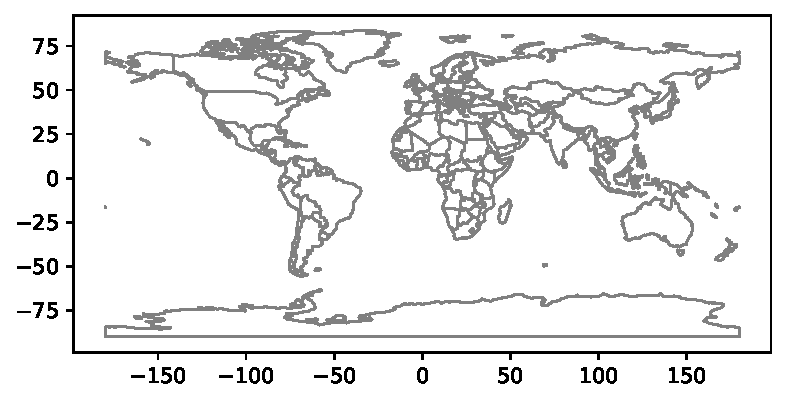
\includegraphics[scale=0.75]{02_times_files/02_times_127_0.pdf}
\end{center}

\begin{center}
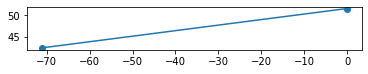
\includegraphics[scale=0.75]{02_times_files/02_times_127_1.png}
\end{center}

The two plots are on different axes, which is not what we want in this
case.

To get the points and the map on the same axes, we have to use a
function from Matplotlib, which is a visualization library we will use
extensively. We'll import it like this.

\begin{lstlisting}[language=Python,style=source]
import matplotlib.pyplot as plt
\end{lstlisting}

The function is \passthrough{\lstinline!gca!}, which stands for ``get
current axes''. We can use the result to tell
\passthrough{\lstinline!plot!} to put the points and lines on the
current axes, rather than create a new one.

\begin{lstlisting}[language=Python,style=source]
ax = plt.gca()
world.plot(color='white', edgecolor='gray', ax=ax)
series.plot(ax=ax);
\end{lstlisting}

\begin{center}
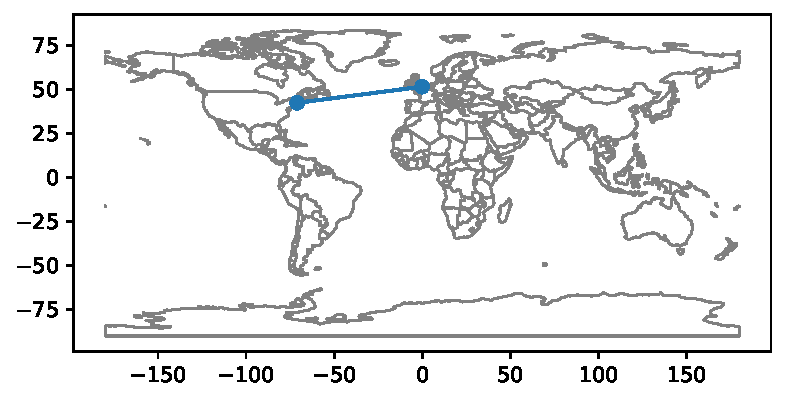
\includegraphics[scale=0.75]{02_times_files/02_times_131_0.pdf}
\end{center}

There are a few features in this example I have not explained
completely, but hopefully you get the idea.

\textbf{Exercise:} Modify the code in this section to plot a point that
shows the home town you chose in a previous exercise and a line from
there to Boston.

